\chapter{Experimentos}\label{chapter:experiments}

\section{Hipótesis a validar}

El objetivo central de este trabajo es validar la hipótesis de que extender las gaussianas empleadas en el algoritmo de \emph{Gaussian Splatting} para incorporar formas asimétricas, mediante la introducción de un parámetro de \emph{skewness}, permite una representación más fiel y expresiva de escenas tridimensionales. A diferencia de las gaussianas tradicionales, que presentan bordes difuminados y simétricos, las gaussianas asimétricas propuestas permiten simular colas alargadas y bordes más definidos, características que podrían ser determinantes en la reconstrucción precisa de superficies con límites abruptos o transiciones de color pronunciadas.

Esta generalización no solo busca mejorar la reconstrucción visual en términos de métricas objetivas como \emph{PSNR}, \emph{SSIM} y \emph{LPIPS}, sino también explorar la posibilidad de que el borde más rígido inducido por la asimetría pueda actuar como una estimación de la normal local a la superficie representada. Tal propiedad podría ser explotada en aplicaciones posteriores, tales como la generación de mallas poligonales a partir de nubes gaussianas, técnicas de sombreado y estimación de iluminación basada en normales. En consecuencia, se pretende evaluar no solo la capacidad de estas gaussianas asimétricas para representar con mayor precisión tanto bordes duros como gradientes suaves, sino también su potencial utilidad como entidades geométricas intermedias en tareas de reconstrucción y renderizado más avanzadas.

\section{Diseño experimental}

La experimentación se ve condicionada por la disponibilidad de recursos computacionales, en particular la imposibilidad de acceder a una GPU con 24\,GB de memoria, cantidad recomendada para la ejecución eficiente de algoritmos de \emph{Gaussian Splatting} sobre conjuntos de datos clásicos como \emph{Mip-NeRF 360} y \emph{Tanks \& Temples}. Por este motivo, se decide la construcción de un conjunto de datos propio, optimizado para un consumo de memoria reducido, que permitia la validación experimental en hardware más modesto sin sacrificar la representatividad de las escenas.

\subsection{UH-Statues Dataset}

El conjunto de datos creado, denominado \textbf{UH-Statues Dataset}, se compone por 7 escenas distintas (\emph{poey}, \emph{owl}, \emph{almamater}, \emph{urn}, \emph{benito}, \emph{humboldt}, \emph{einstein}), cuidadosamente seleccionadas para cubrir tanto ambientes interiores (\emph{urn} y \emph{poey}) como exteriores. En todos los casos, la captura se realiza apuntando la cámara hacia un objeto principal, siendo en su mayoría estatuas localizadas en la Universidad de La Habana: cinco de ellas situadas en la Facultad de Matemática y Computación y una en la Facultad de Física. La selección de escenas se diseña para garantizar diversidad en la iluminación y el fondo, a la vez que se mantenía el enfoque en un único objeto de interés, lo que facilita el entrenamiento y evaluación del algoritmo.

\begin{figure}[htbp]
    \centering
    \includegraphics[width=1.0\textwidth]{Graphics/dataset.png}
    \caption{Escenas del dataset UH-Statues, de izquierda a derecha las escenas: poey, owl, almamater, benito, urn, humboldt, einstein.}
    \label{fig:dataset}
\end{figure}

La captura de los datos se realiza utilizando un \textbf{iPhone 15} en modo video estándar, con resolución 4K a 30\,\emph{fps}, sin aplicar \emph{zoom}, y utilizando exclusivamente la cámara principal, la cual posee una distancia focal de 26\,mm. La duración de cada video no supera el minuto, lo que limita la cantidad de imágenes a procesar y, en consecuencia, reduce significativamente el consumo de memoria durante el entrenamiento del modelo.

\paragraph{Preprocesamiento y reconstrucción}
El pipeline de preprocesamiento para cada escena consiste en los siguientes pasos:
\begin{enumerate}
    \item \textbf{Extracción de imágenes:} De cada video se extraen 2 fotogramas por segundo, obteniendo así un conjunto de imágenes suficientemente representativo de la escena, pero evitando la redundancia asociada a una mayor frecuencia de muestreo.
    \item \textbf{Transformación y escalado:} Las imágenes extraídas son transpuestas para garantizar una orientación uniforme y redimensionadas a un ancho fijo de 1920 píxeles, manteniendo la relación de aspecto original. Esta reducción de resolución es clave para disminuir el consumo de memoria y acelerar el procesamiento subsiguiente.
    \item \textbf{Reconstrucción de la cámara:} La calibración y reconstrucción de la geometría de la escena se realizó utilizando \textbf{COLMAP}, especificando que las imágenes son tomadas con una cámara tipo \emph{pinhole} y distorsión radial/tangencial siguiendo el modelo de OpenCV. COLMAP [\cite{schonberger2016structure}] es una herramienta robusta para la reconstrucción tridimensional a partir de imágenes, que estima tanto las posiciones relativas de las cámaras como una nube de puntos 3D de la escena. El resultado de COLMAP incluye los parámetros intrínsecos y extrínsecos de la cámara para cada imagen, así como una reconstrucción inicial de la estructura 3D, información que posteriormente se emplea como entrada para el algoritmo de \emph{Gaussian Splatting}.
\end{enumerate}

\paragraph{Ventajas de este dataset}
La principal ventaja del \emph{UH-Statues Dataset} radica en su bajo consumo de memoria durante el entrenamiento, consecuencia directa de:
\begin{itemize}
    \item El número reducido de imágenes por escena, derivado tanto de la corta duración de los videos como de la baja frecuencia de muestreo de fotogramas.
    \item La resolución moderada de las imágenes, que limita el tamaño de los mapas de proyección y los buffers intermedios utilizados durante la rasterización.
    \item La simplicidad de las escenas, en las que predomina un único objeto de interés y fondos poco recargados, lo que reduce la necesidad de una gran cantidad de gaussianas para una reconstrucción precisa.
\end{itemize}
Este diseño permite ejecutar el pipeline completo de \emph{Gaussian Splatting} en GPUs con capacidad de memoria limitada, a diferencia de datasets más complejos y de mayor tamaño, como \emph{Mip-NeRF 360}, donde la cantidad de imágenes y la resolución implican requerimientos significativamente más altos.

\section{Métricas de evaluación}

Para cuantificar la calidad de las reconstrucciones obtenidas mediante los diferentes modelos, se emplean las métricas objetivas estándar en la literatura de síntesis y reconstrucción de imágenes: \textbf{PSNR}, \textbf{SSIM} y \textbf{LPIPS}. Estas métricas han demostrado ser indicadores confiables del parecido visual entre la imagen generada y la imagen real, y son ampliamente utilizadas tanto en los trabajos fundacionales de \emph{Gaussian Splatting} [\cite{kerbl20233d}] como en métodos derivados.

\subsection{PSNR (Peak Signal-to-Noise Ratio)}
El \emph{PSNR} es una métrica tradicionalmente utilizada para evaluar la calidad de imágenes reconstruidas, definida en función del error cuadrático medio (\emph{MSE}) entre la imagen generada y la imagen de referencia. Matemáticamente, se expresa como:
\begin{equation}
    \mathrm{PSNR} = 10 \cdot \log_{10} \left( \frac{MAX_I^2}{\mathrm{MSE}} \right)
\end{equation}  

donde $MAX_I$ es el valor máximo posible de un píxel en la imagen. Un mayor valor de PSNR indica mayor similitud entre las imágenes. Esta métrica es sensible a pequeños errores de reconstrucción y ha sido utilizada extensivamente en la literatura de procesamiento de imágenes [\cite{huynh2008scope}].

\subsection{SSIM (Structural Similarity Index)}
El \emph{SSIM} [\cite{wang2004image}] es una métrica perceptual que evalúa la similitud estructural entre dos imágenes, considerando luminancia, contraste y estructura. Se calcula mediante:
\begin{equation}
    \mathrm{SSIM}(x, y) = \frac{(2\mu_x\mu_y + c_1)(2\sigma_{xy} + c_2)}{(\mu_x^2 + \mu_y^2 + c_1)(\sigma_x^2 + \sigma_y^2 + c_2)}
\end{equation}
donde $\mu_x$, $\mu_y$ son las medias, $\sigma_x^2$, $\sigma_y^2$ las varianzas, y $\sigma_{xy}$ la covarianza local de las ventanas comparadas en cada imagen. SSIM produce valores entre $-1$ y $1$, siendo $1$ el máximo de similitud.

\subsection{LPIPS (Learned Perceptual Image Patch Similarity)}
\emph{LPIPS} [\cite{zhang2018unreasonable}] es una métrica aprendida, que mide la distancia perceptual entre imágenes utilizando activaciones intermedias de redes neuronales profundas entrenadas para reconocimiento de imágenes. A diferencia de PSNR y SSIM, LPIPS se correlaciona mejor con la percepción humana de similitud visual, especialmente en contextos de reconstrucción de imágenes complejas o sintéticas. Valores bajos de LPIPS indican mayor similitud perceptual entre la imagen generada y la de referencia.




\section{Resultados Cuantitativos}

Se entrenó un modelo para cada escena del dataset desarrollado, realizando 15000 iteraciones para cada una. En la mayoría de las escenas se aplicó un proceso de densificación cada 100 iteraciones hasta alcanzar las primeras 1000 iteraciones. Excepcionalmente, las escenas denominadas \textit{poey} y \textit{owl} pudieron densificarse hasta la iteración 5000, debido al menor consumo de memoria en la GPU. Todos los experimentos se realizan en una Nvidia RTX 4060 Max-Q de 8\,GB.

La comparación directa entre el método propuesto, \textbf{Directional Asymmetric Gaussian Splatting (DA-GS)}, y el método original, se presenta en la Figura~\ref{tab:quality_dags_vs_vanilla}. Se muestran las métricas Peak Signal-to-Noise Ratio (PSNR), Structural Similarity Index Measure (SSIM), Learned Perceptual Image Patch Similarity (LPIPS), así como el número final de puntos en cada modelo entrenado (Pts).

\begin{table}[h!]
    \centering
    \resizebox{\textwidth}{!}{%
    \begin{tabular}{@{}lcccc cccc@{}}
        \toprule
        & \multicolumn{4}{c}{\textbf{DA-GS}}
        & \multicolumn{4}{c}{\textbf{Vanilla GS}} \\
        \cmidrule(lr){2-5}\cmidrule(lr){6-9}
        Escena & PSNR$\uparrow$ & SSIM$\uparrow$ & LPIPS$\downarrow$ & Pts$\downarrow$
               & PSNR$\uparrow$ & SSIM$\uparrow$ & LPIPS$\downarrow$ & Pts$\downarrow$ \\
        \midrule
        poey       & --    & -- & -- & --         & 33.20 & -- & -- & 2,390,147 \\
        almamater  & 24.45 & -- & -- & \textbf{72,557} & 25.22 & -- & -- & 73,762 \\
        owl        & 24.12 & -- & -- & \textbf{1,356,670} & 24.87 & -- & -- & 2,238,576 \\
        humboldt   & 18.13 & -- & -- & 27,423         & 18.81 & -- & -- & \textbf{26,388} \\
        benito     & 23.68 & -- & -- & \textbf{731,137} & 24.32 & -- & -- & 750,608 \\
        urn        & 27.50 & -- & -- & 22,234         & 30.32 & -- & -- & \textbf{20,604} \\
        einstein   & --    & -- & -- & --             & --    & -- & -- & -- \\
        \bottomrule
    \end{tabular}}
    \caption{Comparación de calidad entre \textbf{DA-GS} y \textbf{Vanilla GS}. Para PSNR y SSIM, valores más altos son mejores ($\uparrow$); para LPIPS y el número final de puntos (Pts) valores más bajos son mejores ($\downarrow$).}
    \label{tab:quality_dags_vs_vanilla}
\end{table}

Además, se realiza una comparación adicional para validar el comportamiento del \textbf{DA-GS} cuando se congela el parámetro de asimetría en 0, esperado a comportarse de manera similar al método original del \textbf{GS}. Estos resultados se presentan en la Figura~\ref{tab:quality_dags_vs_skewfrozen}.

\begin{table}[H]
    \centering
    \resizebox{\textwidth}{!}{%
    \begin{tabular}{@{}lcccc cccc@{}}
        \toprule
        & \multicolumn{4}{c}{\textbf{DA-GS}}
        & \multicolumn{4}{c}{\textbf{DA-GS (skew frozen)}} \\
        \cmidrule(lr){2-5}\cmidrule(lr){6-9}
        Escena & PSNR$\uparrow$ & SSIM$\uparrow$ & LPIPS$\downarrow$ & Pts$\downarrow$
               & PSNR$\uparrow$ & SSIM$\uparrow$ & LPIPS$\downarrow$ & Pts$\downarrow$ \\
        \midrule
        poey       & --    & -- & -- & --             & 32.81 & -- & -- & 2,605,931 \\
        almamater  & \textbf{24.45} & -- & -- & \textbf{72,557}         & 24.43 & -- & -- & 73,698 \\
        owl        & \textbf{24.12} & -- & -- & \textbf{1,356,670}      & 23.71 & -- & -- & 2,165,915 \\
        humboldt   & 18.13 & -- & -- & \textbf{27,423}         & \textbf{18.29} & -- & -- & 28,145 \\
        benito     & 23.68 & -- & -- & 731,137        & --    & -- & -- & -- \\
        urn        & 27.50 & -- & -- & 22,234         & \textbf{27.78} & -- & -- & \textbf{22,051} \\
        einstein   & --    & -- & -- & --             & --    & -- & -- & -- \\
        \bottomrule
    \end{tabular}}
    \caption{Comparación de calidad entre \textbf{DA-GS} y \textbf{DA-GS con skewness congelado}. Para PSNR y SSIM, valores más altos son mejores ($\uparrow$); para LPIPS y Pts valores más bajos son mejores ($\downarrow$).}
    \label{tab:quality_dags_vs_skewfrozen}
\end{table}

\section{Resultados Cualitativos}

Para validar cualitativamente la hipótesis de que las gaussianas con asimetría explotan sus bordes más definidos para modelar bordes en objetos tridimensionales, se procede a colorear las gaussianas según la dirección del vector de asimetría. Estos resultados son comparados visualmente con las normales obtenidas de la implementación original del \textit{Gaussian Splatting}, las cuales son extraídas a partir de la dirección de menor varianza de cada gaussiana. La comparación visual de ambos métodos puede apreciarse en la Figura~\ref{fig:normals}.

\begin{figure}[htbp]
\centering
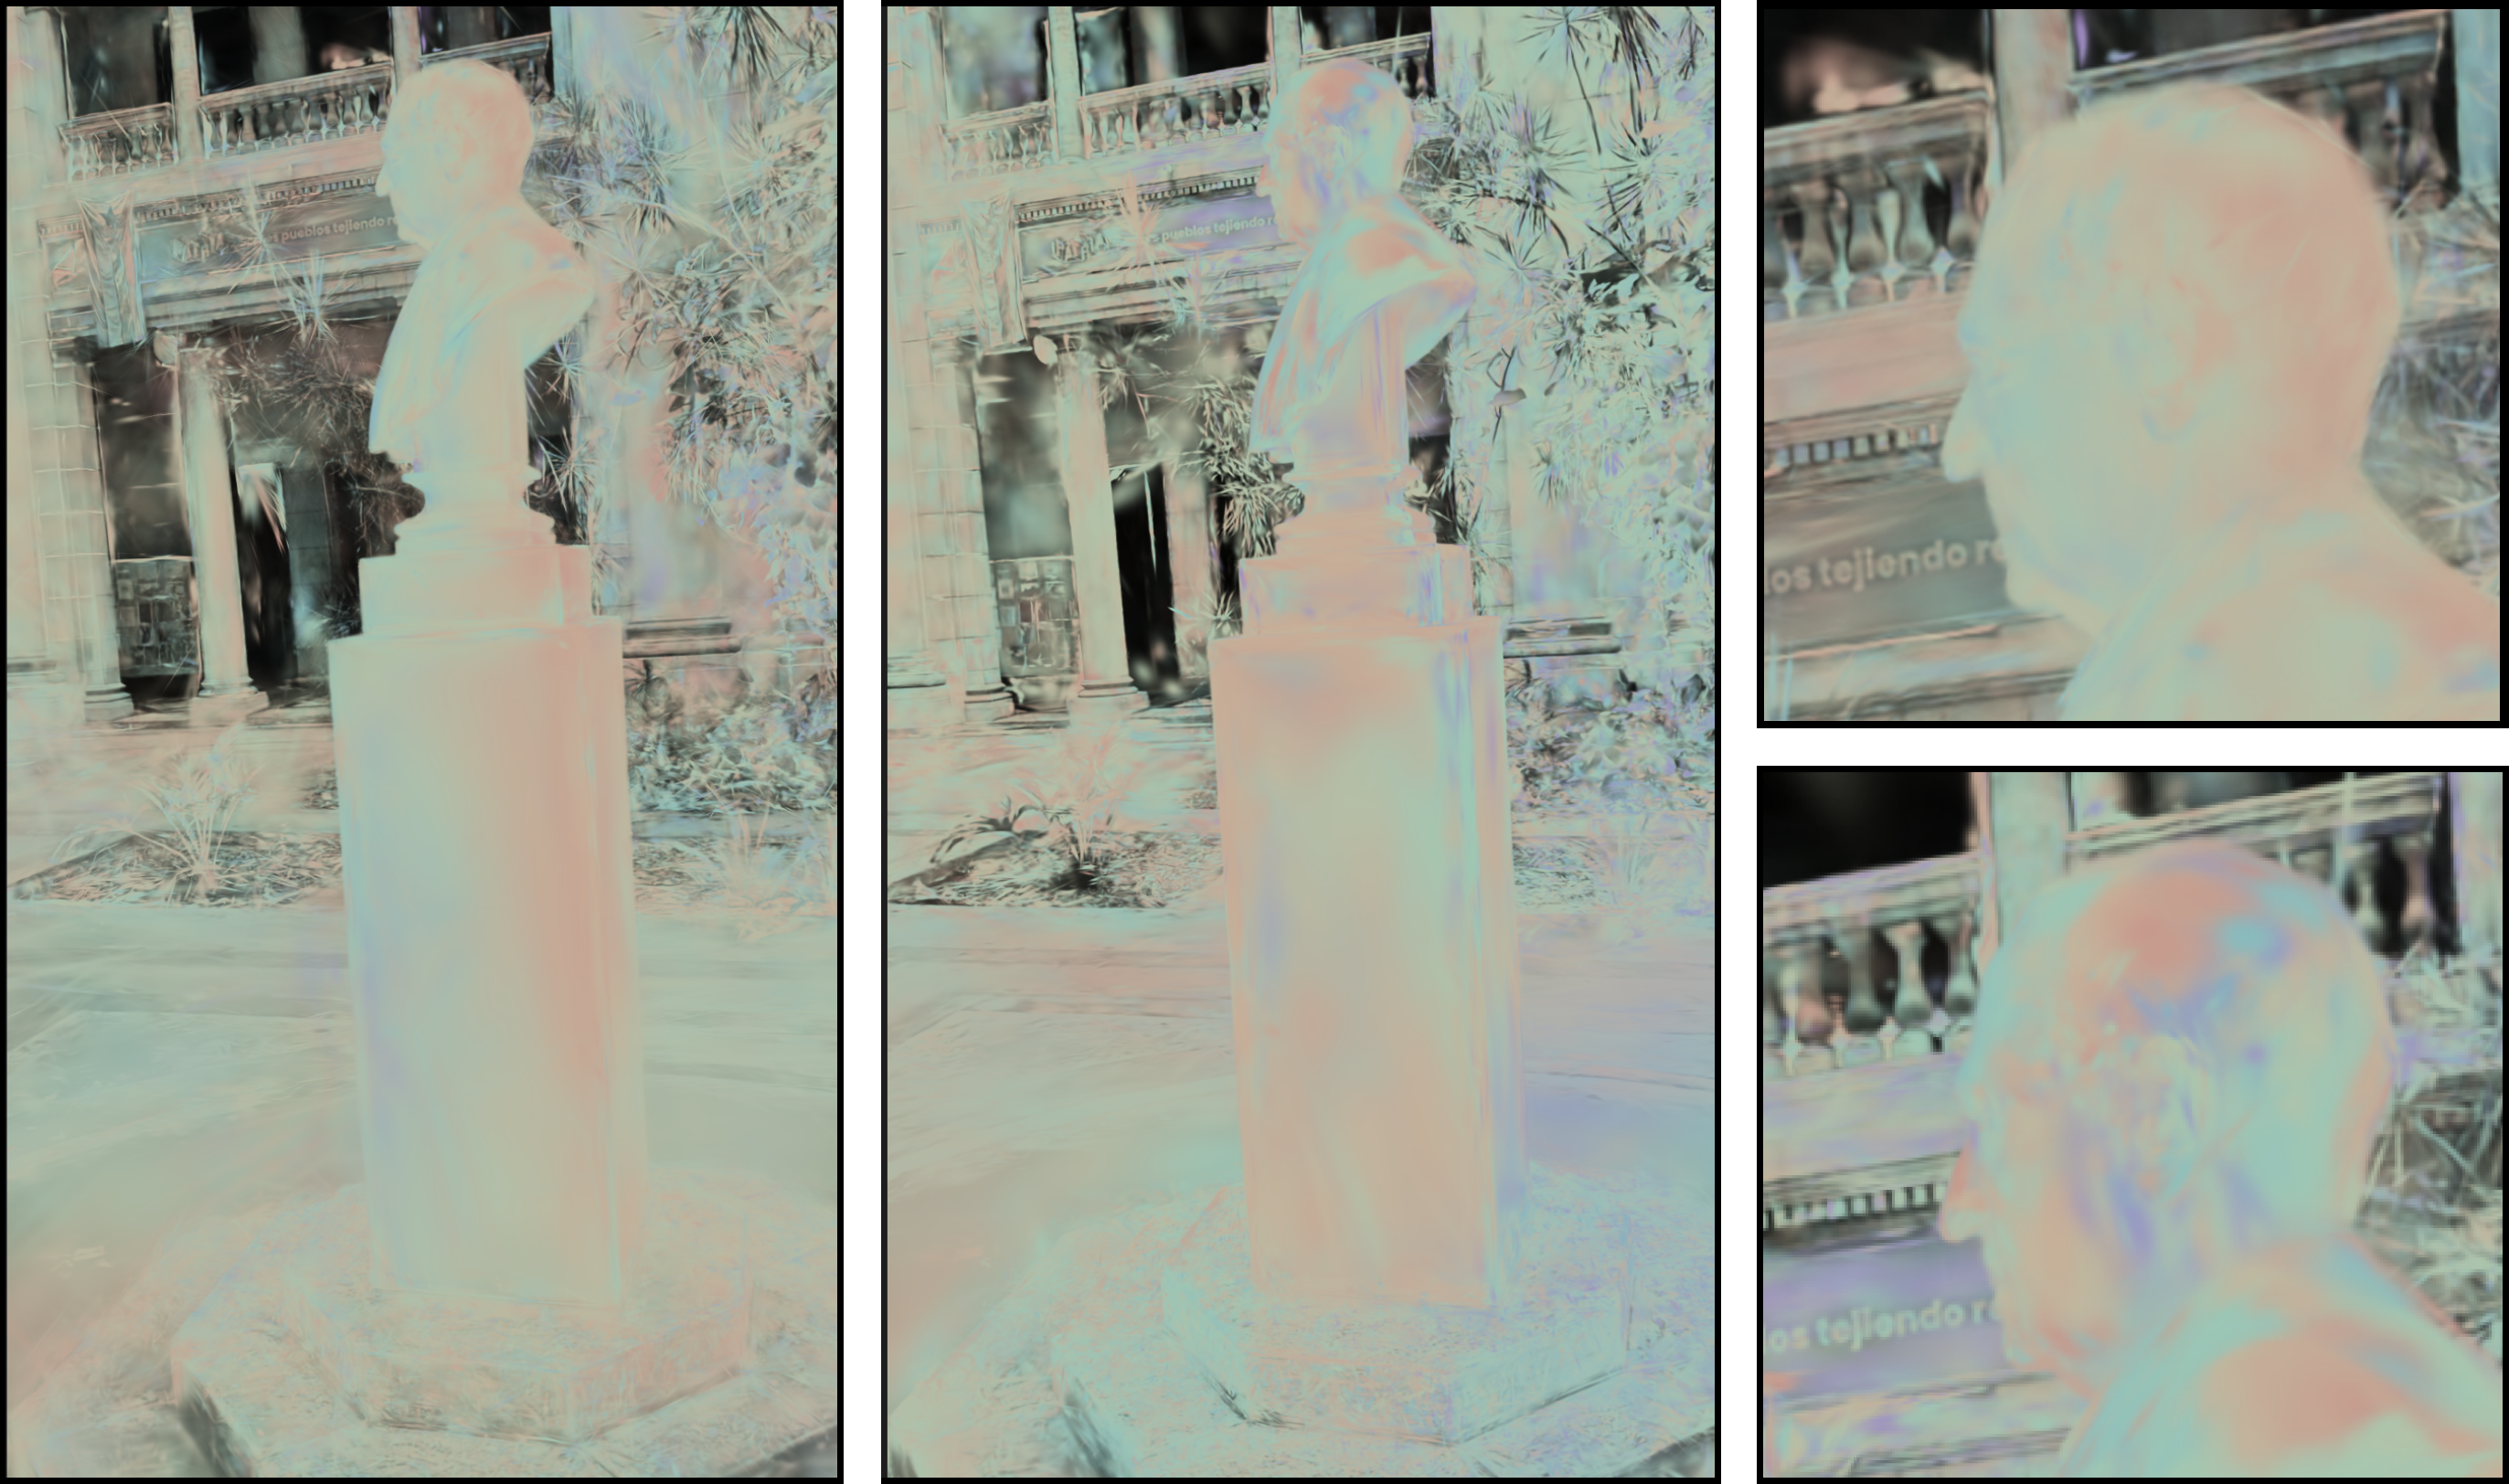
\includegraphics[width=1.0\textwidth]{Graphics/normals.png}
\caption{Comparación visual de la dirección del vector de asimetría (izquierda) y las normales estimadas por el \textit{Gaussian Splatting} original (derecha). Modelos entrenados sobre la escena \textit{poey}, a 5000 iteraciones.}
\label{fig:normals}
\end{figure}

\subsubsection{Análisis y discusión}


Los resultados obtenidos revelan que si bien, en términos absolutos, no se alcanzan los resultados del \textit{Gaussian Splatting} original, se evidencia que la incorporación del parámetro de asimetría aporta beneficios medibles. Al comparar la versión completa del modelo con la variante en la que el parámetro de \textit{skewness} se congela en cero, se observa de manera consistente que el uso de gaussianas asimétricas mejora los resultados. Esto respalda la hipótesis fundamental de este trabajo: que la introducción de direccionalidad permite una mejor adaptación local a la geometría de la escena, particularmente en regiones con bordes o discontinuidades.

Sin embargo, un hallazgo relevante es que incluso al congelar el parámetro de asimetría, con lo cual el modelo debería comportarse de manera análoga al GS original, se obtienen resultados inferiores. Esta observación sugiere que el modelo DA-GS posee dinámicas de entrenamiento diferentes, posiblemente debido a su mayor complejidad y número de parámetros.

Aunque se ha realizado un proceso de ajuste de hiperparámetros, los resultados indican que podrían ser necesarias estrategias de ajuste más específicas, adaptadas a las características particulares del nuevo modelo. En particular, el mayor espacio de búsqueda asociado a la complejidad adicional podría requerir una mayor sensibilidad en la selección de tasas de aprendizaje, esquemas de densificación y regularización.

Además, la inclusión de nuevos parámetros puede introducir inestabilidades numéricas durante el entrenamiento, lo cual también podría afectar la convergencia hacia soluciones óptimas. A pesar de estas dificultades, los resultados cualitativos respaldan la utilidad del \textit{skewness}: las gaussianas tienden a orientar su asimetría hacia los bordes de los objetos, reforzando su definición. Esto sugiere que el \textit{skewness} puede ser aprovechado como una fuente adicional de información geométrica, complementaria a las normales estimadas por el método original. Su potencial utilidad en tareas como iluminación, reconstrucción de mallas o segmentación estructural merece ser explorada en trabajos futuros.

\subsubsection{Limitaciones observadas}

Entre las principales limitaciones identificadas durante los experimentos se destacan las siguientes:

\begin{itemize}
    \item A pesar de su mayor capacidad expresiva, el modelo DA-GS no supera al \textit{Gaussian Splatting} original en las métricas cuantitativas bajo las configuraciones actuales de entrenamiento.
    \item La variante con \textit{skewness} congelado, que teóricamente debería comportarse de manera equivalente al GS tradicional, no logra igualar su desempeño, lo que sugiere diferencias no triviales en la dinámica de optimización.
    \item La complejidad adicional del modelo impone un mayor desafío para la selección de hiperparámetros adecuados y puede introducir inestabilidades numéricas que afecten negativamente la convergencia.
\end{itemize}

A pesar de estas limitaciones, los resultados obtenidos son alentadores. El modelo DA-GS logra reconstrucciones visualmente comparables utilizando una menor cantidad de puntos en varias escenas, lo cual implica un uso más eficiente de los recursos. Por ejemplo, en la escena \textit{owl}, se logró una reconstrucción similar empleando poco más de la mitad de los puntos utilizados por el método original. Este ahorro es significativo si se considera que únicamente se añadieron cuatro parámetros adicionales por gaussiana, las cuales originalmente tienen al menos 59 parámetros (valores de punto flotante).Este comportamiento evidencia que la asimetría no solo enriquece la capacidad representacional del modelo, sino que también puede contribuir a una codificación más compacta y eficiente de la geometría de la escena.

